\section{The question and the results}\label{sec:intro}
A square Ising system is given a boundary at each size determined by the restrictions of one independent sign field on $\Z^2$. Which infinite-volume Gibbs states can one observe along subsequences of \emph{all} square sizes? A preference of order $\sqrt n$ usually selects one pure phase. The question concerns the exceptional sizes at which the two phases have nearly equal free energies. We prove that these sizes realize every mixture weight.

The distinction between recurrence and frequency is essential. The empirical distribution of the finite-volume measures gives mass one half to each pure phase, yet its cluster set contains their entire segment (Figure~\ref{fig:segment}). A sequence can visit every interior neighbourhood infinitely often and spend a vanishing fraction of its time there.

\begin{figure}[ht]
\centering
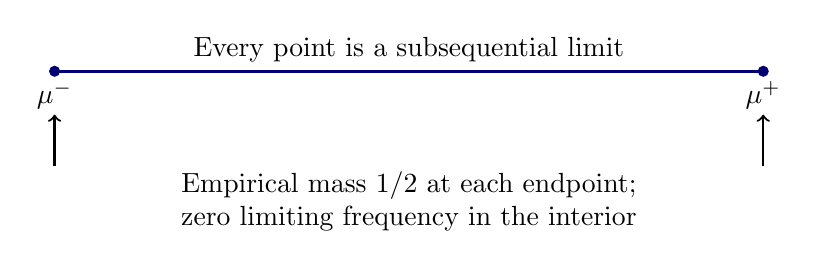
\begin{tikzpicture}[x=9cm,y=1cm]
\draw[very thick,blue!45!black] (0,0)--(1,0);
\fill[blue!45!black] (0,0) circle (2pt) (1,0) circle (2pt);
\node[below] at (0,0) {$\mu^-$};
\node[below] at (1,0) {$\mu^+$};
\node[above] at (.5,0) {Every point is a subsequential limit};
\draw[->,thick] (0,-1.2)--(0,-.55);
\draw[->,thick] (1,-1.2)--(1,-.55);
\node[below,align=center] at (.5,-1.15) {Empirical mass $1/2$ at each endpoint;\\zero limiting frequency in the interior};
\end{tikzpicture}
\caption{The cluster set and the empirical metastate describe different aspects of the same sequence. The drawing records the conclusions, rather than a finite-size probability density.}\label{fig:segment}
\end{figure}

Here is the range of the results. Let $K_c=\tfrac12\log(1+\sqrt2)=0.44068679\ldots$ be the critical inverse temperature of the planar nearest-neighbour model \cite{KW41,Onsager44}. Throughout the main results, $K$ is fixed and finite with $K>K_c$. This is the whole region in which the plus and minus phases coexist (for $K\le K_c$ the spontaneous magnetization vanishes \cite{Yang52,BGJS73} and the Gibbs state is unique \cite{LML72}).

Write $B_n=[-n,n]^2\cap\Z^2$, and let $\mu_n^\eta$ be the zero-field nearest-neighbour Gibbs measure with exterior spins $\eta$ and coupling $K$ on every bond meeting $B_n$. The signs $\eta_x$ are independent with $\Pp_p(\eta_x=+1)=p$. Let $\mu^\pm$ be the pure phases, $a_\pm=\mu^\pm(\sigma_0=+1)$, $m=a_+-a_->0$, and
\[
 \nu_\lambda=\lambda\mu^++(1-\lambda)\mu^-,\qquad
 X_n=\mu_n^\eta(\sigma_0=+1),\qquad
 T_n=\frac{X_n-a_-}{m}.
\]
The topology on states is local weak convergence.

The main assertion concerns the complete sequence of integers.
\begin{maintheorem}[Every mixture recurs]\label{thm:cluster}
Let $K>K_c$ and $p=1/2$. Almost surely the weak cluster set of $(\mu_n^\eta)_{n\ge1}$ is exactly $\{\nu_\lambda:0\le\lambda\le1\}$.
\end{maintheorem}

The quantitative ingredient is a lower bound in arbitrarily narrow fixed windows.
\begin{maintheorem}[The local-window lower bound]\label{thm:lower}
Let $K>K_c$. For every $0<u<v<1$ there are $c=c(K,u,v)>0$ and $n_0=n_0(K,u,v)$ such that
\[
 \Pp_{1/2}(u<T_n<v)\ge c n^{-1/2}\qquad(n\ge n_0).
\]
For every weakly open neighbourhood $\mathcal U$ of any $\nu_\lambda$ with $0<\lambda<1$, the same lower bound holds for $\Pp_{1/2}(\mu_n^\eta\in\mathcal U)$, with constants depending on $K$, $\mathcal U$ and $\lambda$.
\end{maintheorem}

Bias selection and the empirical law complete the picture.
\begin{maintheorem}[Biased and fair laws]\label{thm:laws}
Let $K>K_c$. For each fixed $p>1/2$, almost surely $\mu_n^\eta\Rightarrow\mu^+$ along all sizes; for $p<1/2$ the limit is $\mu^-$. For $p=1/2$, almost surely
\[
 \frac1N\sum_{n=1}^N\delta_{\mu_n^\eta}
 \Rightarrow\tfrac12\delta_{\mu^+}+\tfrac12\delta_{\mu^-},
 \qquad \frac1N\sum_{n=1}^N X_n\longrightarrow\tfrac12.
\]
\end{maintheorem}

\paragraph{Position in the literature.}
Theorem~\ref{thm:cluster} proves the two-dimensional conjecture of van Enter, Neto\v cn\'y and Schaap \cite[Remark~3.2]{vENS05}, stated there for sufficiently large $K$, at every $K>K_c$. An earlier form is due to van Enter, Medved' and Neto\v cn\'y \cite{EMN02}, for weak boundary couplings. In the frozen-bulk model they found countably many null-recurrent mixtures along all cubes in dimensions two and three. They conjectured that every mixture is an almost-sure limit point at finite low temperature, and they identified a lower bound of order $n^{-(d-1)/2-\zeta}$ on fixed-interval free-energy probabilities as the missing step \cite[Sections~1 and~6]{EMN02}. The 2005 paper's Theorem~3.1 concerns sufficiently sparse sizes, and its Theorem~3.4 gives the empirical endpoint law at sufficiently low temperature. We recover the latter conclusion at every $K>K_c$, the full range in which \cite[Section~1]{vENS05}, following \cite{NS92}, expected the finite-volume states to oscillate between the two phases. Their Proposition~3.5 bounds probabilities of fixed local departures from both phases by $O(n^{-1/2+\alpha})$, at a temperature threshold depending on $\alpha>0$. Wherever that threshold holds, Theorem~\ref{thm:lower} supplies the lower half of the order $n^{-1/2}$ that their Remark~3.6 conjectures and places beyond their technique. The upper bound retains that published temperature hypothesis. The 2006 note \cite[Section~3]{vENS06} explains the same recurrence and metastate distinction; its Remark~3.2 expects every mixture to be a null-recurrent limit point and names the missing lower bounds on small free-energy differences as the obstacle. Higuchi's Theorem~1 \cite{Higuchi78} already gives the selection of Theorem~\ref{thm:laws}, on his boxes, for independent boundaries with $p<3/8$ or $p>5/8$ at sufficiently low temperature; his Theorem~2 shows that boundary density alone does not decide the phase above $3/8$. For tuned deterministic boundary conditions every mixture is already a weak limit of square Gibbs states: Gallavotti \cite{Gallavotti72} obtained the symmetric mixture from Dobrushin boundary conditions at low temperature, Messager and Miracle-Sol\'e \cite{MMS77} extended this to all $K>K_c$, and Abraham and Reed \cite{AbrahamReed76} obtained every $\nu_\lambda$ by shifting the Dobrushin interface (see \cite[Section~1.1.1]{Coquille15}); Theorem~\ref{thm:cluster} shows that boundaries which are not tuned, typical independent fair words, realize every mixture along the sequence of all squares.

\begin{table}[ht]
\centering\small
\begin{tabular}{@{}>{\raggedright\arraybackslash}p{.23\textwidth}>{\raggedright\arraybackslash}p{.35\textwidth}>{\raggedright\arraybackslash}p{.34\textwidth}@{}}
\toprule
Question & Prior result & Result here, every $K>K_c$\\
\midrule
Cluster set & Pure endpoints along sufficiently sparse sizes \cite[Theorem~3.1]{vENS05}; countably many mixtures for the frozen bulk \cite{EMN02} & Whole segment along every integer size\\
Interior-window probability & Upper bound $O(n^{-1/2+\alpha})$ \cite[Proposition~3.5]{vENS05} & Lower bound $c n^{-1/2}$\\
Empirical metastate & Equal endpoint masses \cite[Theorem~3.4]{vENS05} & Recovery throughout the ordered phase\\
Biased boundaries & Boundary plus-density below $3/8$ selects $\mu^-$ at sufficiently low temperature \cite[Theorem~1]{Higuchi78}; related settings \cite{EMN02,CampaninoEnter}, \cite[Section~2]{vENS06} & Every fixed $p\ne1/2$: almost-sure convergence along all squares\\
\bottomrule
\end{tabular}
\caption{The model in the main results has independent exterior spins and boundary bonds of the bulk strength. Published existential thresholds in the middle column keep their original hypotheses.}\label{tab:landscape}
\end{table}

Newman and Stein introduced chaotic size dependence, raising the random-boundary Ising question in \cite{NS92}, and developed the empirical metastate viewpoint \cite{NewmanStein}; Aizenman and Wehr provided the disorder-based metastate construction \cite{AizenmanWehr}. The classification of planar DLR states is due to Aizenman and Higuchi \cite{Aizenman,Higuchi81}; we use its finite-volume form due to Coquille and Velenik \cite{CV}. Earlier work on boundary-driven phase selection includes Higuchi \cite{Higuchi78}, Campanino and van Enter \cite{CampaninoEnter} for the Potts model at its transition temperature, and Higuchi and Yoshida \cite{HY97}; see also \cite[Section~2]{vENS06}. Endo, van Enter and Le Ny review random boundary conditions in \cite{EEL19}. Their 2024 work \cite{EEL24} obtains mixed-state metastates in one-dimensional long-range models, a related phenomenon in a different interaction geometry. Our proof rests on inputs valid throughout the ordered phase: the random-line representation of the dual high-temperature model developed by Pfister and Velenik \cite{PV97,PV99}, surface-order large deviations of the magnetization \cite{Ioffe95,Schonmann87,CCS87}, the spatial relaxation of \cite{BLP81,CCS87}, and the wetting theory of Fr\"ohlich and Pfister \cite{FP1,FP2}.

\paragraph{Reading guide and proof idea.}
Section~\ref{sec:model} fixes the model and the published inputs. Section~\ref{sec:dual} writes the model with its physical boundary in terms of open dual arcs: the boundary word determines their endpoints, reversing a boundary interval prices any family of arcs, and fixing all open arcs leaves pure-boundary Ising laws. Section~\ref{sec:contours} shows that macroscopic arcs are rare for typical boundaries, that the sign of the spin sum in a central square labels the phase, and that the two ensembles conditioned on this sign are separated near the north side. Section~\ref{sec:odds} identifies their log odds with the phase weight. The main new lower bound is in Section~\ref{sec:windows}: a long constant-sign boundary buffer makes each selected change arbitrarily small, while many such changes still move the mean odds by order $n$. Counting their crossings of a fixed window gives $n^{-1/2}$. Section~\ref{sec:laws} proves recurrence, bias selection and frequencies. Readers interested in the probability argument can take Section~\ref{sec:dual}, the pure-phase inputs and uniform-wall uniqueness of Section~\ref{sec:model} as black boxes.
